\documentclass[12pt,a4paper]{article}
\usepackage{amsmath}
\usepackage{graphicx}
\usepackage{hyperref}
\usepackage[utf8]{inputenc}
\usepackage[english, greek]{babel}
\usepackage{listings}
\usepackage{xcolor}

\title{Αναφορά: Μετρητές Morris και Βελτιστοποίηση Εκτίμησης Πλήθους}
\author{Εργαστήριο Αλγοριθμικών Τεχνικών}
\date{}


\begin{document}


\maketitle


\section{Εισαγωγή στους Μετρητές Morris}


Οι μετρητές Morris αποτελούν μια καινοτόμο προσέγγιση για την εκτίμηση του πλήθους στοιχείων σε ροές δεδομένων με περιορισμένη μνήμη. Βασικό χαρακτηριστικό τους είναι η χρήση μιας στοχαστικής μεθόδου για την καταμέτρηση, όπου η πιθανότητα αύξησης του μετρητή μειώνεται εκθετικά.


\subsection{Βασική Υλοποίηση Μετρητή Morris}


Ο κλασικός μετρητής Morris ορίζεται από τον ακόλουθο ψευδοκώδικα:

\selectlanguage{english}
\begin{lstlisting}[
  language=Pascal,
  caption={Basic Morris Counter Algorithm},
  captionpos=b,
  frame=single,
  basicstyle=\ttfamily\small,
  commentstyle=\color{green!50!black},
  keywordstyle=\color{blue!70!black},
  backgroundcolor=\color{gray!10}
]
// Initialize counter
integer C = 0

// Insert element
void insert() {
    // Increment with decreasing probability
    C <- C+1, with probability 1/2^C
}

// Estimate count
integer query() {
    return 2^C - 1
}
\end{lstlisting}
\selectlanguage{greek}


Βασικά χαρακτηριστικά:
\begin{itemize}
\item Χαμηλή απαίτηση μνήμης (περίπου 4-5 bits για $n = 1.000.000$)
\item Στοχαστική προσέγγιση εκτίμησης
\item Μη γραμμική συμπεριφορά αύξησης μετρητή
\end{itemize}


\subsection{Βελτιστοποιημένος Μετρητής Morris}


Προτείναμε δύο βελτιστοποιήσεις στον βασικό αλγόριθμο:


\begin{enumerate}
\item \textbf{Πολλαπλοί Μετρητές:} Χρήση 5 ανεξάρτητων μεταβλητών C
\begin{itemize}
\item Μέθοδος Μέσου Όρου: $(2^{C_1} + 2^{C_2} + ... + 2^{C_5} - 5)/5$
\item Μέθοδος Διαμέσου: Υπολογισμός διαμέσου των $2^{C_i} - 1$
\end{itemize}


\item \textbf{Παραμετροποίηση με $\alpha$:} Αντί για σταθερή βάση 2, χρησιμοποιήσαμε $1 \leq \alpha \leq 2$
\begin{itemize}
    \item Εκτίμηση: $\frac{1}{\alpha-1}(\alpha^C - 1)$
    \item Βέλτιστο $\alpha \approx 1.14$ για 8 bits και $n = 1.000.000$
\end{itemize}

\end{enumerate}


\section{Αποτελέσματα και Ανάλυση}


\subsection{Σύγκριση Μεθόδων}


\begin{figure}[h!]
\centering
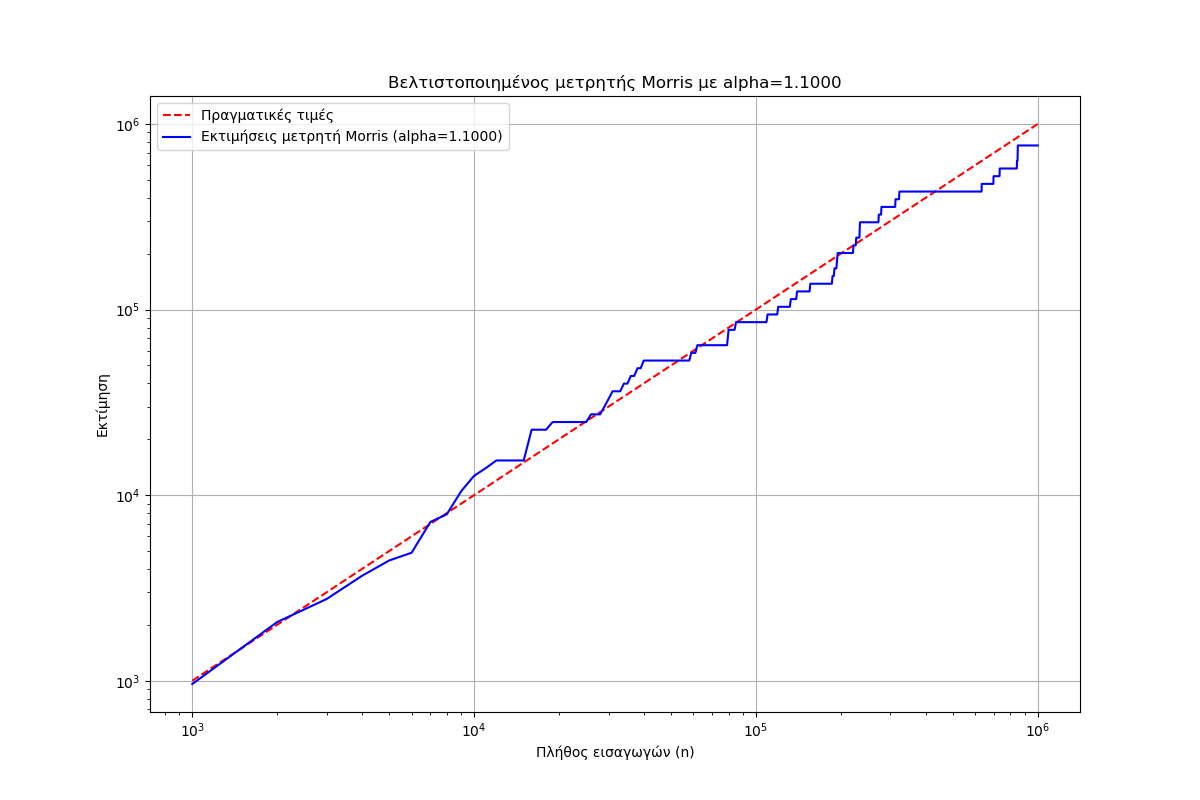
\includegraphics[width=0.8\textwidth]{optimized_morris_counter.png}
\caption{Εκτίμηση πλήθους με βελτιστοποιημένο μετρητή Morris ($\alpha = 1.14$)}
\end{figure}


Κύρια συμπεράσματα:
\begin{itemize}
\item Το βέλτιστο $\alpha$ μειώνει το σχετικό σφάλμα εκτίμησης
\item Μέσος όρος και διάμεσος παρέχουν σταθερότερες εκτιμήσεις
\item Η μέθοδος διαμέσου είναι ανθεκτικότερη σε ακραίες τιμές
\end{itemize}


\section{Συμπεράσματα}


Οι μετρητές Morris προσφέρουν:
\begin{itemize}
\item Πολύ χαμηλή κατανάλωση μνήμης
\item Δυνατότητα εκτίμησης μεγάλων συνόλων
\item Ευελιξία μέσω παραμετροποίησης
\end{itemize}


Προτάσεις για περαιτέρω έρευνα περιλαμβάνουν τη διερεύνηση προσαρμοστικών μεθόδων επιλογής παραμέτρων και σύγκριση με άλλες τεχνικές προσέγγισης πλήθους.


\end{document}